Pour chaque question, recopier sur la copie son numéro et la réponse correspondante.

Pour cette partie, aucune justification n'est demandée.

Pour les questions à choix multiple, une seule réponse est exacte.

\subsection*{Question 1}
L'écriture scientifique du nombre \np{45310} est :

\begin{tblr}{colspec={*{4}{|X[c]}|},hlines}
	\textbf{A.}\quad $45,31 \times 10^{3}$ &
	\textbf{B.}\quad $4,531 \times 10^{4}$ &
	\textbf{C.}\quad $4,531 \times 10^{-4}$ &
	\textbf{D.}\quad $4531 \times 10^{1}$\\
\end{tblr}

\subsection*{Question 2}
Une forme développée de l'expression $(4x-3)(4x+3)$ est :

\begin{tblr}{colspec={*{4}{|X[c]}|},hlines}
	\textbf{Réponse A} & \textbf{Réponse B} & \textbf{Réponse C} & \textbf{Réponse D} \\
	$4x^2 - 9$ & $16x^2+9$ & $16x^2-9$ & $8x^2-6$
\end{tblr}

\subsection*{Question 3}
Un pavé droit a pour dimensions : 4,5 cm de long, 4 cm de large, 10 cm de haut. Le volume de ce pavé est de :

\begin{tblr}{colspec={*{4}{|X[c]}|},hlines}
	\textbf{Réponse A} & \textbf{Réponse B} & \textbf{Réponse C} & \textbf{Réponse D} \\
	$180~\text{cm}^3$ & $170~\text{cm}^3$ & $160,5~\text{cm}^3$ & $18,5~\text{cm}^3$
\end{tblr}

\subsection*{Question 4}
On considère les nombres suivants et on s'intéresse à leur divisibilité par 9.

\[N = \np{2025} \quad \text{et} \quad P = \np{2026}.\]

\begin{tblr}{colspec={*{4}{|X[c]}|},hlines}
	\textbf{Réponse A} & \textbf{Réponse B} & \textbf{Réponse C} & \textbf{Réponse D} \\
	\small $N$ et $P$ sont tous les deux divisibles par 9 & $N$ est divisible par 9 mais $P$ ne l'est pas & $P$ est divisible par 9 mais $N$ ne l'est pas & Aucun des deux n'est divisible par 9
\end{tblr}

\subsection*{Question 5}
Une personne a couru 9~km en 45~minutes.

Quelle est sa vitesse moyenne en km/h ?

\subsection*{Question 6}

\begin{minipage}{0.68\textwidth}
	Une roue de la fortune est utilisée pour faire gagner des cadeaux. La roue est divisée en 10 secteurs de tailles égales, avec les gains suivants : des stylos, des porte-clés, des casques audios ou un smartphone.

	Un joueur tourne la roue une seule fois.

	Quelle est la probabilité que le joueur gagne un casque audio ?
\end{minipage}%
\hfill
\begin{minipage}{0.28\textwidth}
	\centering
	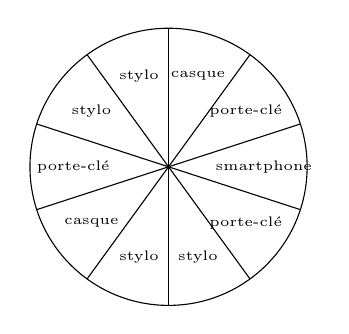
\begin{tikzpicture}[scale=1.1]
		\foreach \i in {0,...,9} {
			\draw (0,0) -- (90+36*\i:1.6);
		}
		\draw (0,0) circle (1.6);
		\node at (108:1.1) {\tiny stylo};
		\node at (72:1.1) {\tiny casque};
		\node at (36:1.1) {\tiny porte-clé};
		\node at (0:1.1) {\tiny smartphone};
		\node at (-36:1.1) {\tiny porte-clé};
		\node at (-72:1.1) {\tiny stylo};
		\node at (-108:1.1) {\tiny stylo};
		\node at (-144:1.1) {\tiny casque};
		\node at (180:1.1) {\tiny porte-clé};
		\node at (144:1.1) {\tiny stylo};
	\end{tikzpicture}
\end{minipage}

\subsection*{Question 7}
Un article coûte 60 \euro. Calculer son nouveau prix après une baisse de 10\,\%.

\subsection*{Question 8}

\begin{minipage}{0.62\textwidth}
	Quelle est la mesure de l'angle $\widehat{\text{BAC}}$ ?
\end{minipage}%
\hfill
\begin{minipage}{0.34\textwidth}
	\centering
	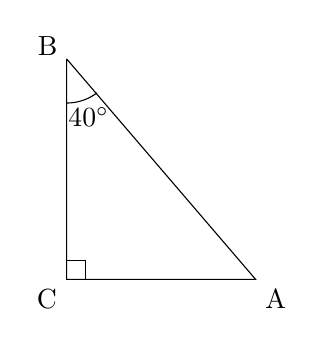
\begin{tikzpicture}[scale=0.8]
		\coordinate (C) at (0,0);
		\coordinate (A) at (3,0);
		\coordinate (B) at (0,3.5);
		\draw (B) -- (C) -- (A) -- (B);
		\draw (0,0.3) -- (0.3,0.3) -- (0.3,0);
		\node at (-0.3,3.7) {B};
		\node[below left] at (C) {C};
		\node[below right] at (A) {A};
		\draw (0,2.8) arc(-90:-53:0.8) node[pos=0.7, below]{$40^\circ$};
	\end{tikzpicture}
\end{minipage}

\subsection*{Question 9}
Le diagramme en barres ci-dessous donne les notes des élèves d'une classe au dernier contrôle de mathématiques.

\begin{enumerate}[label=\textbf{\alph*.}]
	\item Combien d'élèves ont participé à ce contrôle ?
	\item Quelle est la note médiane ?
\end{enumerate}

\begin{center}
	%Début Tikz
	%\begin{tikzpicture}
	%\begin{axis}[
	%  ybar,
	%  width=15cm,
	%  height=6cm,
	%  bar width=12pt,
	%  xlabel={notes},
	%  ylabel={effectif},
	%  symbolic x coords={7,8,9,10,11,12,13,14,15,16,17,18},
	%  xtick=data,
	%  ymin=0, ymax=6,
	%  ytick={0,1,2,3,4,5,6},
	%  enlarge x limits=0.05,
	%  axis lines=left,
	%  nodes near coords,
	%]
	%\addplot coordinates {(7,3) (8,4) (10,4) (11,5) (12,5) (15,3) (17,2) (18,1)};
	%\end{axis}
	%\end{tikzpicture}
	%Fin Tikz
	% Début PSTricks
	\psset{unit=0.9cm,arrowsize=2pt 3}
	\begin{pspicture}(-1,-1)(12.5,6.5)
		\psaxes[linewidth=1.25pt,Ox=6]{->}(0,0)(0,0)(12.5,6.5)
		\psframe(0.8,0)(1.2,3)\psframe(1.8,0)(2.2,4)\psframe(3.8,0)(4.2,4)
		\psframe(4.8,0)(5.2,5)\psframe(5.8,0)(6.2,5)\psframe(8.8,0)(9.2,3)
		\psframe(10.8,0)(11.2,2)\psframe(11.8,0)(12.2,1)
		\rput(6,-0.8){notes}\rput{90}(-0.8,3.25){effectifs}
	\end{pspicture}
	%Fin PSTricks
\end{center}
